\chapter{DISCUSSÃO TRANSVERSAL}
\label{chap:discussao}

\section{Resposta às perguntas de pesquisa}

\subsection{Preservação do ranking}

A primeira pergunta investigou em que medida os rankings que emergem do treinamento dos classificadores nos braços sintéticos reproduzem o ranking completo dos subconjuntos no braço real. Os resultados mostram que essa preservação pode ser elevada mesmo quando as amostras sintéticas não reproduzem visualmente a distribuição real. Em $n=512$, 19 das 20 comparações sintéticas apresentadas nas Tabelas~\ref{tab:occupancy-final}, \ref{tab:air-final}, \ref{tab:support2-original} e \ref{tab:support2-rf} obtiveram $\rankrho$ superior a $0{,}79$, e várias ultrapassaram $0{,}95$.

O ranking é particularmente importante para decisões de eficiência porque não depende apenas da identidade do primeiro colocado. Ele revela se subconjuntos de menor custo permanecem próximos do topo, se alternativas quase equivalentes são ordenadas de modo semelhante e se canais aparentemente redundantes mantêm posição inferior nos diferentes braços. A resposta à RQ1 é, portanto, positiva para grande parte das configurações, mas a intensidade da preservação varia com o cenário.

\subsection{Preservação das relações de vencedores}

A segunda pergunta tratou das relações par a par resumidas pela \WinnersAgreement{}. Essa métrica acompanhou de perto a correlação de ranking, mas não é redundante com ela. Spearman mede a associação entre posições; a Winners Agreement mede diretamente a proporção de pares para os quais os dois braços concordam sobre qual subconjunto possui menor perda.

Os valores finais foram elevados em todos os cenários, com destaque para Gaussian Naive Bayes no Air Quality e no Occupancy. A interpretação operacional é direta: um valor de $0{,}95$ significa que aproximadamente 95\% das comparações válidas entre configurações mantiveram a mesma decisão de superioridade. Isso é mais informativo para custo e eficiência do que exigir a coincidência exata do primeiro colocado, especialmente quando vários subconjuntos apresentam perdas muito próximas.

\subsection{Preservação dos limiares de vantagem cooperativa}

A RQ3 recebeu uma resposta mais heterogênea. A similaridade progressiva de \Nstar{} foi, em geral, menor que ranking e Winners Agreement. O resultado é esperado porque a métrica exige concordância simultânea sobre a existência dos cruzamentos e sobre a posição de seu último evento. Pequenas perturbações nas curvas podem deslocar um cruzamento entre potências de dois sem alterar de forma importante a ordenação final.

A variação observada foi ampla: de $0{,}2087$ no SVM do Air Quality com Gaussiana única a $0{,}8085$ no Gaussian Naive Bayes do mesmo dataset com GMM. Isso demonstra que a fidelidade de \Nstar{} não é uma consequência automática de ranking alto. No Occupancy, por exemplo, o Gaussian Naive Bayes com Gaussiana única obteve $\rankrho=0{,}9976$ e $A_W=0{,}9892$, mas similaridade de \Nstar{} de apenas $0{,}2452$.

\subsection{Evolução com o tamanho amostral}

A RQ4 pergunta como a preservação evolui com $n$. As curvas publicadas mostram oscilações mais frequentes nos menores tamanhos amostrais, quando a variabilidade de estimação é maior. Em muitos casos, ranking e Winners Agreement aumentam ou se estabilizam conforme novos dados são adicionados. A similaridade de \Nstar{} pode apresentar comportamento menos monotônico, pois cada novo prefixo acrescenta eventos, atualiza últimos cruzamentos e altera simultaneamente o conjunto de células e a normalização temporal.

Não se deve formular uma lei universal de crescimento. O resultado defensável é mais restrito: nos experimentos avaliados, a instabilidade estrutural esteve concentrada principalmente em regimes de pequenas amostras, enquanto os indicadores de ordenação tenderam a se tornar mais estáveis em $n$ maiores. As exceções e oscilações permanecem relevantes, sobretudo em datasets de baixa separabilidade e classificadores com curvas irregulares.

\subsection{Dependência do classificador}

A RQ5 é respondida claramente: a preservação depende do classificador. Amostras produzidas pelo mesmo gerador podem induzir estruturas muito diferentes quando muda a regra de decisão usada no treinamento. No Air Quality, Gaussian Naive Bayes apresentou preservação quase perfeita do ranking e dos vencedores, enquanto o SVM teve similaridade de \Nstar{} bastante menor. No SUPPORT2, o Random Forest reproduziu os últimos cruzamentos melhor que SVM, regressão logística e Gaussian Naive Bayes, apesar de sua perda elevada.

Esse resultado reforça que a fidelidade não é propriedade isolada do gerador. O objeto avaliado é a interação entre distribuição de treinamento, subconjunto de canais, classificador e teste real. Uma distribuição sintética pode ser adequada para estudar a cooperação de um classificador e inadequada para outro.

\subsection{Dependência do gerador}

A RQ6 também recebe resposta condicionada. O GMM não venceu de forma uniforme. Ele melhorou a similaridade de \Nstar{} em todas as configurações de Occupancy e Air Quality, mas perdeu para a Gaussiana única no Random Forest do SUPPORT2. Para ranking e Winners Agreement, houve casos em que a Gaussiana única foi superior, especialmente no SVM do Occupancy.

A conclusão relevante não é que o GMM seja melhor, mas que a complexidade adicional deve ser justificada pelo tipo de estrutura que se deseja reproduzir. Quando o treinamento com amostras da Gaussiana única alcança resultados próximos ou superiores, o gerador simples é preferível por ser mais leve, mais interpretável e potencialmente mais acessível a análises matemáticas. O GMM é útil quando o treinamento com suas amostras produz ganho estrutural substantivo, e não apenas maior semelhança visual.

\section{Preservação multidimensional}

Os resultados rejeitam uma concepção binária de fidelidade. Um braço pode preservar a ordenação global, concordar na maioria das decisões par a par e ainda deslocar os limiares de \Nstar{}. Também pode preservar uma matriz densa de últimos cruzamentos mesmo sem produzir boa classificação absoluta. Dessa forma, cada configuração deve ser descrita por um perfil:
\[
\left(
  \rankrho(n),
  A_W(n),
  \mathrm{NS}(n),
  \overline{L}(n)
\right).
\]

Esse perfil evita dois erros. O primeiro seria declarar que um modelo ``falhou'' apenas porque não recuperou exatamente o primeiro subconjunto ou todos os cruzamentos. O segundo seria declarar que um modelo ``preservou a cooperação'' com base somente em uma correlação alta. A utilidade depende do objetivo: ordenação de alternativas, comparação de custos, decisão entre pares ou previsão do regime em que uma configuração se torna vantajosa.

\section{Fidelidade geométrica e fidelidade estrutural}

O Occupancy oferece o contraste mais claro entre aparência e estrutura. O GMM produz nuvens visualmente mais próximas dos dados reais, mas a Gaussiana única obteve melhor ranking e Winners Agreement no SVM em $n=512$. A consequência metodológica é importante: avaliar geradores somente por histogramas, projeções ou distâncias distributivas pode conduzir a uma conclusão diferente daquela obtida quando o objeto de interesse é uma decisão do classificador.

A geometria continua relevante. Air Quality e SUPPORT2 apresentam regiões mais compatíveis com aproximações gaussianas em parte de suas projeções, e isso pode ajudar a explicar a alta preservação observada em determinadas combinações. Entretanto, três datasets são insuficientes para estabelecer uma relação causal. O presente estudo fornece hipóteses: regularidade geométrica, sobreposição entre classes, dependência entre canais e hipótese do classificador parecem interagir com a fidelidade estrutural. Testar essas associações exigirá um conjunto maior de problemas e descritores geométricos quantitativos.

\section{Desempenho preditivo e preservação estrutural}

O Random Forest do SUPPORT2 separa de forma particularmente clara desempenho absoluto e estrutura relativa. A menor perda ficou próxima de $0{,}455$, pouco abaixo do erro majoritário de $0{,}4687$. Ainda assim, a similaridade de \Nstar{} alcançou $0{,}6799$ e $0{,}6340$, superando todos os demais classificadores daquele dataset.

Esse resultado não é explicado por escassez de cruzamentos. As matrizes possuíam mais de onze mil células dirigidas com evento definido, e mais de dez mil eram compartilhadas entre a referência e cada braço sintético. A interpretação mais plausível é que o Random Forest respondeu de maneira consistente às vantagens \emph{relativas} dos subconjuntos, mesmo sem extrair informação suficiente para uma separação absoluta forte entre as classes.

A distinção pode ser organizada em quatro quadrantes conceituais, apresentados na Figura~\ref{fig:conceito-quadrante}.

\begin{figure}[H]
  \centering
  \caption{Relação conceitual entre desempenho preditivo absoluto e preservação da estrutura de cooperação}
  \label{fig:conceito-quadrante}
  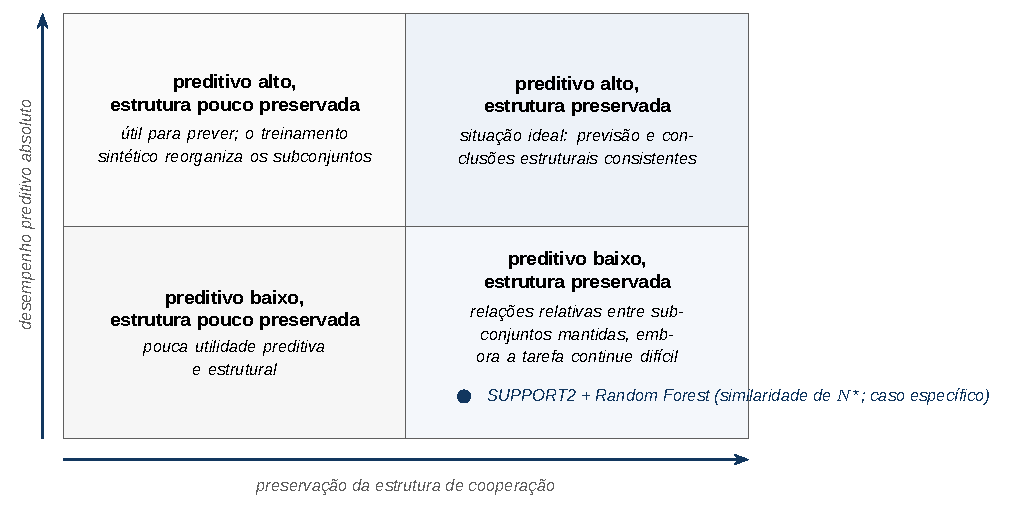
\includegraphics[width=0.95\textwidth]{figures/conceptual/quadrante_desempenho.pdf}
  \sourcebelow{elaboração própria}
  \notailustracao{A posição do caso SUPPORT2 com Random Forest refere-se à similaridade de $\Nstar$ observada nesse cenário específico e não deve ser generalizada para outros datasets ou classificadores.}
\end{figure}

O Random Forest do SUPPORT2 ocupa o quadrante de desempenho preditivo baixo com estrutura preservada, em relação à similaridade de \Nstar{}. Isso não torna o classificador adequado para uso clínico, nem valida decisões operacionais. Mostra apenas que baixa perda e fidelidade estrutural são critérios distintos e que o simulador deve reportá-los separadamente.

\section{O papel da simplicidade}

A preferência inicial por uma Gaussiana única não decorre da expectativa de que ela seja universalmente mais precisa. Ela decorre de seu menor custo de parametrização e amostragem, de sua interpretabilidade e da possibilidade de desenvolver análises matemáticas sobre médias e covariâncias. Se o treinamento com amostras de um modelo simples reproduz a organização relevante, adicionar componentes ao GMM pode trazer pouco benefício científico.

Os resultados oferecem exemplos nos dois sentidos. No SVM do Occupancy, o treinamento com amostras da Gaussiana única reproduziu melhor o ranking e os vencedores. No Gaussian Naive Bayes do Air Quality, as estruturas obtidas com amostras de ambos os geradores foram praticamente idênticas à referência nessas métricas, tornando a solução simples especialmente atraente. Por outro lado, o treinamento com amostras do GMM aumentou de forma relevante a similaridade de \Nstar{} em várias configurações. O princípio resultante é de parcimônia condicionada: usar o modelo mais simples cujas amostras, após o treinamento do classificador, reproduzam os componentes estruturais necessários para a decisão.

\section{Limites da interpretação de \texorpdfstring{$\Nstar$}{N*}}

A escolha do último cruzamento torna \Nstar{} útil para representar a transição final observada, mas não descreve toda a dinâmica. Dois braços podem concordar sobre o último evento e divergir em cruzamentos intermediários; podem também apresentar trajetórias de perda muito diferentes antes da estabilização. Portanto, alta similaridade de \Nstar{} não deve ser descrita como reprodução integral das curvas.

Ao mesmo tempo, a regra do último cruzamento é operacionalmente defensável quando se deseja saber a partir de qual regime a relação final disponível se estabelece. Em curvas com múltiplas inversões, o primeiro cruzamento poderia sugerir vantagem prematura. O último evento é mais conservador, desde que o relatório deixe explícito o limite da grade e a possibilidade de novas inversões fora do intervalo observado.

\section{Relação com a literatura}

O comportamento de subconjuntos maiores em pequenas amostras é compatível com o fenômeno de Hughes e com a literatura sobre efeitos de tamanho amostral em reconhecimento de padrões \cite{hughes1968,raudys1991}. A diferença entre relevância individual, redundância e utilidade conjunta também se alinha à literatura de seleção de variáveis \cite{guyon2003,brown2012}. O CoInfoSim se distingue por acompanhar todos os subconjuntos ao longo de uma grade de $n$ e por avaliar se essa organização é preservada quando o treinamento passa de real para sintético.

O protocolo de treinamento sintético e teste real dialoga com avaliações TSTR \cite{esteban2017}, mas desloca o foco da utilidade preditiva agregada para a fidelidade estrutural. Essa mudança explica por que um cenário como SUPPORT2 com Random Forest permanece cientificamente informativo mesmo quando a perda é alta.

Finalmente, a motivação operacional se relaciona à classificação sensível a custos e à seleção de sensores \cite{turney1995,turney2002,joshi2009}. O presente trabalho ainda não resolve um problema econômico. Ele fornece os objetos necessários para essa extensão: rankings, relações par a par, curvas de perda e limiares de transição. O próximo capítulo discute como esses objetos podem ser incorporados a modelos de custo específicos de cada domínio.
